\documentclass[
11pt, % The default document font size, options: 10pt, 11pt, 12pt
%codirector, % Uncomment to add a codirector to the title page
]{charter} 

% Para usar tablas con formato tabularx que permiten seguir en la página siguiente.
\usepackage{ltablex}
\keepXColumns


% El títulos de la memoria, se usa en la carátula y se puede usar el cualquier lugar del documento con el comando \ttitle
\titulo{Sistema de telemetría y detección de eventos para motocicletas} 

% Nombre del posgrado, se usa en la carátula y se puede usar el cualquier lugar del documento con el comando \degreename
\posgrado{Carrera de Especialización en Sistemas Embebidos} 
%\posgrado{Carrera de Especialización en Internet de las Cosas} 
%\posgrado{Carrera de Especialización en Inteligencia Artificial}
%\posgrado{Maestría en Sistemas Embebidos} 
%\posgrado{Maestría en Internet de las cosas}

% Tu nombre, se puede usar el cualquier lugar del documento con el comando \authorname
% IMPORTANTE: no omitir titulaciones ni tildación en los nombres, también se recomienda escribir los nombres completos (tal cual los tienen en su documento)
\autor{Ing. Tomás Enrique Botalla}

% El nombre del director y co-director, se puede usar el cualquier lugar del documento con el comando \supname y \cosupname y \pertesupname y \pertecosupname
\director{Esp. Ing. Germán Eloy Cardozo}
\pertenenciaDirector{UNLAM} 
\codirector{} % para que aparezca en la portada se debe descomentar la opción codirector en los parámetros de documentclass
\pertenenciaCoDirector{}

% Nombre del cliente, quien va a aprobar los resultados del proyecto, se puede usar con el comando \clientename y \empclientename
\cliente{Jurado CESE}
\empresaCliente{FIUBA}
 
\fechaINICIO{28 de abril de 2026}		%Fecha de inicio de la cursada de GdP \fechaInicioName
\fechaFINALPlan{16 de junio de 2026} 	%Fecha de final de cursada de GdP
\fechaFINALTrabajo{mes de diciembre 2026}	%Fecha de defensa pública del trabajo final


\begin{document}

\maketitle
\thispagestyle{empty}
\pagebreak


\thispagestyle{empty}
{\setlength{\parskip}{0pt}
\tableofcontents{}
}
\pagebreak


\section*{Registros de cambios}
\label{sec:registro}


\begin{table}[ht]
\label{tab:registro}
\centering
\begin{tabularx}{\linewidth}{@{}|c|X|c|@{}}
\hline
\rowcolor[HTML]{C0C0C0} 
Revisión & \multicolumn{1}{c|}{\cellcolor[HTML]{C0C0C0}Detalles de los cambios realizados} & Fecha      \\ \hline
0      & Creación del documento                                 &\fechaInicioName \\ \hline
1      & Se completa hasta el punto 5 inclusive                & {10} de {mayo} de 2026 \\ \hline
2      & Se completa hasta el punto 9 inclusive                & {17} de {mayo} de 2026 \\ \hline
3      & Se completa hasta el punto 12 inclusive                & {24} de {mayo} de 2026 \\ \hline
%4      & Se completa el plan	                                 & {día} de {mes} de 202X \\ \hline

% Si hay más correcciones pasada la versión 4 también se deben especificar acá

\end{tabularx}
\end{table}

\pagebreak



\section*{Acta de constitución del proyecto}
\label{sec:acta}

\begin{flushright}
Buenos Aires, \fechaInicioName
\end{flushright}

\vspace{2cm}

Por medio de la presente se acuerda con el \authorname\hspace{1px} que su Trabajo Final de la \degreename\hspace{1px} se titulará ``\ttitle'' y consistirá en el desarrollo de un sistema embebido de adquisición, registro y transmisión en tiempo real de datos de telemetría para motocicletas. El trabajo tendrá un presupuesto preliminar estimado de 600 horas y un costo estimado de \$ 45.270.000, con fecha de inicio el \fechaInicioName\hspace{1px} y fecha de presentación pública en el \fechaFinalName.

Se adjunta a esta acta la planificación inicial.

\vfill

% Esta parte se construye sola con la información que hayan cargado en el preámbulo del documento y no debe modificarla
\begin{table}[ht]
\centering
\begin{tabular}{ccc}
\begin{tabular}[c]{@{}c@{}}Dr. Ing. Ariel Lutenberg \\ Director posgrado FIUBA\end{tabular} & \hspace{2cm} & \begin{tabular}[c]{@{}c@{}}\clientename \\ \empclientename \end{tabular} \vspace{2.5cm} \\ 
\multicolumn{3}{c}{\begin{tabular}[c]{@{}c@{}} \supname \\ Director del Trabajo Final\end{tabular}} \vspace{2.5cm} \\
\end{tabular}
\end{table}


\section{1. Descripción técnica-conceptual del proyecto a realizar}
\label{sec:descripcion}

El proyecto consiste en el desarrollo de un sistema embebido de adquisición, registro y transmisión de telemetría para motocicletas. El dispositivo está diseñado para capturar variables cinemáticas, ambientales y eléctricas, con un enfoque mixto entre el monitoreo de la conducción y la documentación de rutas.

El mismo se encuadra como un emprendimiento personal en el marco del Trabajo Final de la Carrera de Especialización en Sistemas Embebidos (CESE) de la Facultad de Ingeniería de la Universidad de Buenos Aires (FIUBA). La motivación principal surge de la dificultad que enfrentan los motociclistas para acceder a datos precisos sobre su estilo de manejo y el comportamiento dinámico de su vehículo sin recurrir a equipos de alta competición costosos.

En comparación con el estado del arte actual, donde estos sistemas suelen ser costosos y están orientados casi exclusivamente a la competición profesional, esta solución destaca por su accesibilidad y su capacidad de integración. A diferencia de los dispositivos comerciales estándar que se limitan al registro de posición y velocidad, la propuesta integra variables cinemáticas como el ángulo de inclinación, y el estado eléctrico y térmico del vehículo en un solo equipo.

Para abordar esta problemática, el proyecto propone combinar la captura de datos con la transmisión de telemetría en vivo, funcionando como una caja negra que preserva la ubicación exacta y los parámetros dinámicos previos a un incidente.

El sistema centraliza la información de múltiples sensores mediante interfaces de comunicación comunes (\textit{Inter-Integrated Circuit} (I2C), \textit{Serial Peripheral Interface} (SPI), \textit{Universal Asynchronous Receiver-Transmitter} (UART)). Sus funciones principales incluyen:

\begin{itemize}
    \item Registro de ruta y visualización de viajes: utiliza un módulo \textit{Global Positioning System} (GPS) para obtener posición y velocidad con alta precisión. Estos datos permiten generar mapas de recorrido dinámicos en una aplicación móvil, permitiendo al usuario analizar su trayectoria y velocidad en cada tramo.
    \item Detección de eventos críticos: registra caídas, maniobras bruscas (aceleración/frenado) e inclinaciones excesivas. Al detectar un evento, el sistema lo registra para su posterior análisis.
    \item Análisis dinámico: captura datos de una IMU (Inertial Measurement Unit) y un barómetro para estimar ángulos de inclinación, aceleración y altitud.
    \item Gestión de datos: registra la información en una tarjeta \textit{microSD} mediante un esquema de \textit{double buffering} y transmite vía Bluetooth a una aplicación móvil.
    \item Robustez y autonomía: incluye un \textit{watchdog} para recuperación automática ante fallos y modos de bajo consumo para optimizar el uso de la batería de la moto.
\end{itemize}

En la figura \ref{fig:diagBloques} se presenta el diagrama en bloques del sistema. Se observa un microcontrolador encargado de coordinar la lectura de todos los sensores y escribir hacia las diferentes salidas del sistema.

\begin{figure}[htpb]
\centering 
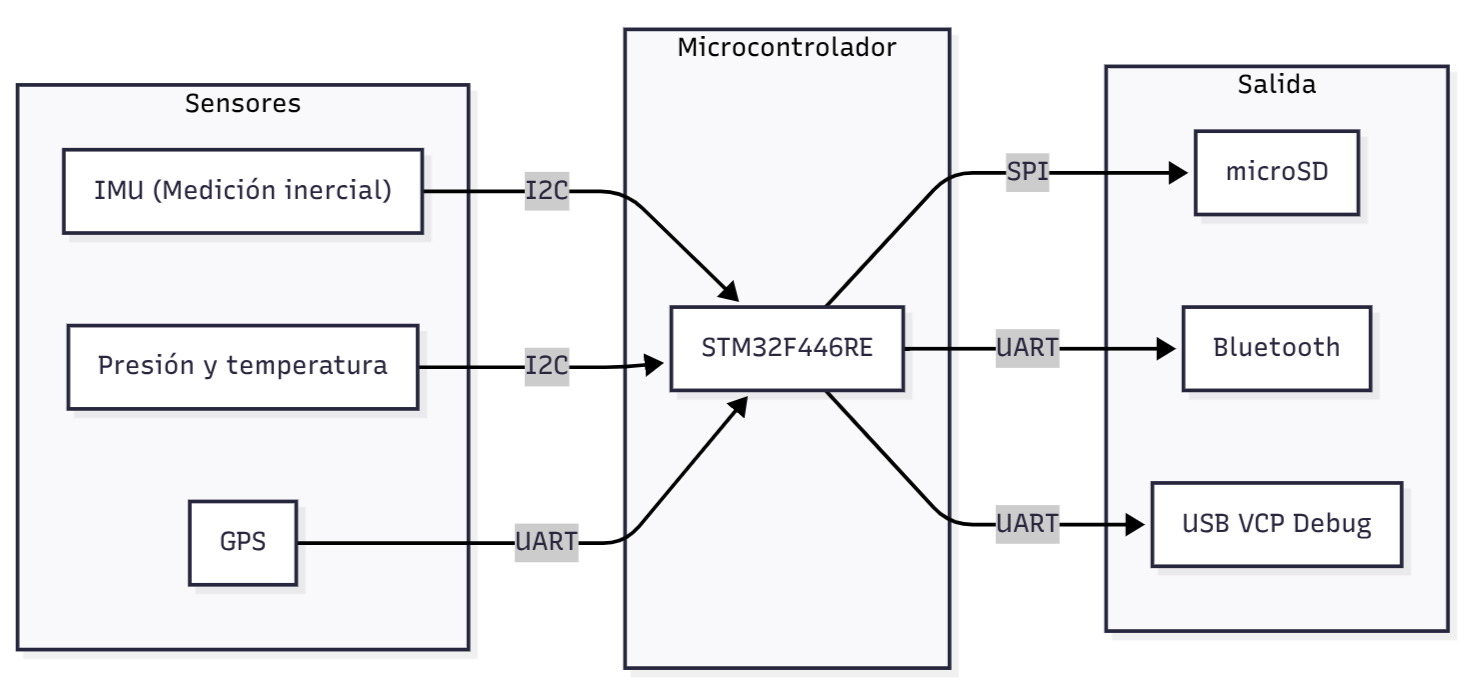
\includegraphics[width=.65\textwidth]{./Figuras/Diagrama bloques.png}
\caption{Diagrama en bloques del sistema.}
\label{fig:diagBloques}
\end{figure}

\section{2. Identificación y análisis de los interesados}
\label{sec:interesados}

\begin{table}[ht]
%\caption{Identificación de los interesados}
%\label{tab:interesados}
\begin{tabularx}{\linewidth}{@{}|l|X|X|l|@{}}
\hline
\rowcolor[HTML]{C0C0C0} 
Rol           & Nombre y Apellido & Organización 	& Puesto 	\\ \hline
%Auspiciante   &                   &              	&        	\\ \hline
Cliente       & \clientename      &\empclientename	& Jurado del CESE       	\\ \hline
%Impulsor      &                   &              	&        	\\ \hline
Responsable   & \authorname       & FIUBA        	& Alumno 	\\ \hline
%Colaboradores &                   &              	&        	\\ \hline
Orientador    & \supname	      & \pertesupname 	& Director del Trabajo Final \\ \hline
%Equipo        & \authorname       & FIUBA            & Alumno       	\\ \hline
%Opositores    & -                 & -            	& -       	\\ \hline
Usuario final & Conductores de motocicletas & -             	& -       	\\ \hline
\end{tabularx}
\end{table}

\section{3. Propósito del proyecto}
\label{sec:proposito}

Desarrollar un sistema embebido de adquisición de datos que permita a los motociclistas analizar su conducción mediante el registro de variables cinemáticas, ambientales y eléctricas. El objetivo es cubrir la escasez de dispositivos de telemetría accesibles que integren la medición de ángulos de inclinación, el monitoreo térmico y eléctrico del vehículo, y el registro de rutas mediante tecnología GPS para la visualización de trayectos en tiempo real e históricos.

\section{4. Alcance del proyecto}
\label{sec:alcance}

El proyecto incluye:

\begin{itemize}
	\item Estudio y selección de sensores.
	\item Diseño y desarrollo del firmware: basado en el microcontrolador \textit{STM32F446RE}, implementando una máquina de estados finita para la gestión del sistema.
	\item Optimización de recursos del microcontrolador: uso de \textit{double buffering} para asegurar el registro en la microSD sin pérdida de datos y \textit{Direct Memory Access} (DMA) para reducir el consumo.
	\item Lógica para la detección de eventos críticos (aceleraciones y frenadas bruscas) y el cálculo de \textit{scoring} de conducción.
	\pagebreak
	\item Desarrollo de una aplicación móvil que se comunique por Bluetooth para visualizar telemetría en tiempo real y mapas de recorrido.
	\item Pruebas
		\begin{itemize}
		\item Unitarias de los manejadores de los sensores.
		\item De integración.
		\item Funcionales.
		\end{itemize}
	\item Documentación técnica del sistema.
		
	
\end{itemize}


El proyecto no incluye:
\begin{itemize}
	\item Conectividad a Internet: el sistema se limita a la transmisión local vía Bluetooth.
	\item Diseño y fabricación de un \textit{Printed Circuit Board} (PCB): el prototipo se desarrollará utilizando módulos comerciales cableados.
	\item El diseño ni la fabricación de un gabinete para el dispositivo.
\end{itemize}

\section{5. Supuestos del proyecto}
\label{sec:supuestos}

Para el desarrollo del presente proyecto se supone que:

\begin{itemize}
	\item El responsable del proyecto, \authorname, cuenta con la dedicación horaria necesaria para cumplir con la planificación y ejecución del mismo.
	\item Al tratarse de un emprendimiento personal, el responsable del proyecto actuará también como el auspiciante, garantizando la disponibilidad del presupuesto para la adquisición de los componentes de hardware.
	\item Los componentes electrónicos a utilizar se podrán adquirir en el mercado local o internacional en tiempo y forma para no demorar las etapas del mismo.
	\item Se dispondrá de una unidad de prueba (motocicleta) que permita la validación funcional del sistema.
	\item El usuario final contará con un dispositivo móvil para la visualización de la información de telemetría.
	\item El responsable del proyecto, \authorname, solo se ausentará de manera indefinida en caso de enfrentar una situación de fuerza mayor.
\end{itemize}

\pagebreak

\section{6. Requerimientos}
\label{sec:requerimientos}

Los requerimientos se agrupan por afinidad y se priorizan según su aporte al objetivo del proyecto.

\begin{enumerate}
	\item Requerimientos funcionales:
		\begin{enumerate}
			\item El sistema debe registrar datos de una IMU en una tarjeta microSD con marca de tiempo. Prioridad: alta.
			\item El sistema debe registrar datos de presión atmosférica provenientes del barómetro. Prioridad: alta.
			\item El sistema debe registrar latitud, longitud y velocidad provistas por el módulo GPS. Prioridad: alta.
			\item El sistema debe registrar la temperatura medida por el sensor seleccionado. Prioridad: media.
			\item El sistema debe detectar eventos críticos de conducción, tales como aceleraciones, frenadas bruscas e inclinaciones excesivas. Prioridad: alta.
			\item El sistema debe transmitir por Bluetooth los datos del recorrido hacia una aplicación móvil. Prioridad: alta.
			\item La aplicación móvil debe mostrar la posición actual en un mapa y los datos principales del recorrido. Prioridad: alta.
			\item La aplicación móvil debe permitir cargar un archivo exportado de un recorrido para visualizarlo sin conexión con la motocicleta. Prioridad: media.
		\end{enumerate}
	\item Requerimientos de firmware y arquitectura embebida:
		\begin{enumerate}
			\item El firmware debe ejecutarse sobre un microcontrolador \textit{STM32F446RE}. Prioridad: alta.
			\item El firmware debe organizar la gestión del sistema mediante una máquina de estados finita. Prioridad: alta.
			\item El firmware debe implementar un esquema de \textit{double buffering} para evitar pérdida de datos durante la escritura en microSD. Prioridad: alta.
			\item El firmware debe contemplar el uso de DMA para reducir la carga de CPU en lecturas de IMU y recepción GPS. Prioridad: media.
			\item El firmware debe incluir un \textit{watchdog} para recuperación automática ante fallos. Prioridad: media.
		\end{enumerate}
	\item Requerimientos de prueba y documentación:
		\begin{enumerate}
			\item Se deben realizar pruebas unitarias de los manejadores de sensores. Prioridad: alta.
			\item Se deben realizar pruebas de integración entre sensores, almacenamiento y transmisión Bluetooth. Prioridad: alta.
			\item Se deben realizar pruebas funcionales en una unidad de prueba. Prioridad: alta.
			\item Se debe generar documentación técnica del sistema desarrollado. Prioridad: alta.
		\end{enumerate}
\end{enumerate}

\section{7. Historias de usuarios (\textit{Product backlog})}
\label{sec:backlog}

Para estimar el esfuerzo relativo entre historias se decidió utilizar story points. Cada historia se evalúa en tres dimensiones, cada una con un peso según la siguiente tabla:

\begin{itemize}
  \item \textbf{Dificultad} (cantidad de trabajo a realizar): bajo → 1, medio → 3, alto → 5.
  \item \textbf{Complejidad} (nivel de sofisticación del trabajo): bajo → 1, medio → 5, alto → 13.
  \item \textbf{Incertidumbre} (riesgo o falta de experiencia en la tarea): bajo → 2, medio → 3, alto → 5.
\end{itemize}

La suma de los tres pesos se aproxima al número de Fibonacci más cercano (1, 2, 3, 5, 8, 13, 21) para obtener el story point final. Como referencia de 1 story point se considera el esfuerzo de integrar un sensor en bus I2C y establecer la comunicación con el microcontrolador.

\begin{itemize}
    \item HU1: como responsable del proyecto, quiero un archivo de texto almacenado en una microSD con datos de la IMU para validar el funcionamiento de la misma.
    \begin{itemize}
      \item Prioridad: alta
      \item Story points: 8 (dificultad: medio(3), complejidad: medio(5), incertidumbre: bajo(2); suma: 10 $\approx$ 8)
    \end{itemize}
    \item HU2: como responsable del proyecto, quiero un archivo de texto almacenado en una microSD con datos del barómetro para validar el funcionamiento del mismo.
    \begin{itemize}
      \item Prioridad: alta
      \item Story points: 5 (dificultad: bajo(1), complejidad: bajo(1), incertidumbre: medio(3); suma: 5)
    \end{itemize}
    \item HU3: como responsable del proyecto, quiero un archivo de texto almacenado en una microSD con latitud, longitud y velocidad para validar el GPS.
    \begin{itemize}
      \item Prioridad: alta
      \item Story points: 8 (dificultad: medio(3), complejidad: medio(5), incertidumbre: bajo(2); suma: 10 $\approx$ 8)
    \end{itemize}
    \item HU4: como responsable del proyecto, quiero un archivo de texto almacenado en una microSD con datos de temperatura, para validar el funcionamiento del sensor.
    \begin{itemize}
      \item Prioridad: media
      \item Story points: 5 (dificultad: bajo(1), complejidad: bajo(1), incertidumbre: medio(3); suma: 5)
    \end{itemize}
    \item HU5: como responsable del proyecto, quiero obtener las lecturas de la IMU usando DMA hacia un buffer en RAM, para reducir el trabajo de la CPU.
    \begin{itemize}
      \item Historia opcional
      \item Prioridad: media
      \item Story points: 8 (dificultad: medio(3), complejidad: medio(5), incertidumbre: bajo(2); suma: 10 $\approx$ 8)
    \end{itemize}
    \item HU6: como responsable del proyecto, quiero obtener las lecturas del GPS usando DMA hacia memoria, para reducir el trabajo de la CPU.
    \begin{itemize}
      \item Historia opcional
      \item Prioridad: media
      \item Story points: 8 (dificultad: medio(3), complejidad: medio(5), incertidumbre: bajo(2); suma: 10 $\approx$ 8)
    \end{itemize}
    \item HU7: como responsable del proyecto, quiero grabar en una microSD los datos de la IMU y el GPS usando doble buffer en RAM y escritura hacia la microSD, para asegurar que los datos no se pierdan.
    \begin{itemize}
      \item Prioridad: alta
      \item Story points: 13 (dificultad: alto(5), complejidad: medio(5), incertidumbre: medio(3); suma: 13)
    \end{itemize}
    \item HU8: como usuario, quiero ver en la aplicación móvil los datos del recorrido en tiempo real, para monitorear el viaje mientras circulo.
    \begin{itemize}
      \item Prioridad: alta
      \item Story points: 8 (dificultad: medio(3), complejidad: medio(5), incertidumbre: bajo(2); suma: 10 $\approx$ 8)
    \end{itemize}
    \item HU9: como usuario, quiero ver en la aplicación móvil la posición actual en un mapa, para ubicarme en la ruta.
    \begin{itemize}
      \item Prioridad: alta
      \item Story points: 8 (dificultad: bajo(1), complejidad: medio(5), incertidumbre: medio(3); suma: 9 $\approx$ 8)
    \end{itemize}
    \item HU10: como usuario, quiero cargar en la aplicación móvil un archivo de texto exportado de un recorrido y visualizar sus datos, para revisar viajes ya grabados sin conexión en tiempo real con la motocicleta.
    \begin{itemize}
      \item Prioridad: media
      \item Story points: 5 (dificultad: bajo(1), complejidad: bajo(1), incertidumbre: medio(3); suma: 5)
    \end{itemize}
    \item HU11: como usuario, quiero ver en el mapa los tramos donde hubo aceleraciones o frenadas bruscas, para localizar esas maniobras en el trayecto.
    \begin{itemize}
      \item Prioridad: alta
      \item Story points: 5 (dificultad: bajo(1), complejidad: bajo(1), incertidumbre: medio(3); suma: 5)
    \end{itemize}
    \item HU12: como responsable del proyecto, quiero investigar las decisiones técnicas y documentar el diseño, la validación y los resultados, para asegurar la trazabilidad del desarrollo y facilitar la revisión del trabajo final.
    \begin{itemize}
      \item Prioridad: alta
      \item Story points: 13 (dificultad: alto(5), complejidad: medio(5), incertidumbre: medio(3); suma: 13)
    \end{itemize}
\end{itemize}

\section{8. Entregables principales del proyecto}
\label{sec:entregables}

Los entregables principales del proyecto son:

\begin{itemize}
	\item Código fuente documentado del sistema embebido para el microcontrolador \textit{STM32F446RE}.
	\item Aplicación móvil para visualización de telemetría en tiempo real y recorridos almacenados.
    \item Documentación técnica del sistema.
    \item Informe de pruebas y validaciones.
    \item Informes de avance del trabajo final.
    \item Prototipo funcional (hardware).
	\item Memoria del trabajo final.
\end{itemize}

\section{9. Desglose del trabajo en tareas}
\label{sec:wbs}

\begin{enumerate}
	\item Investigación (100 h)
	\begin{enumerate}
		\item Selección detallada de componentes y módulos comerciales (25 h)
		\item Análisis de hojas de datos de sensores y microcontrolador (25 h)
		\item Estudio de protocolos de comunicación y almacenamiento (25 h)
		\item Revisión de bibliotecas de soporte y ejemplos de integración (25 h)
	\end{enumerate}
	\item Diseño del sistema (90 h)
	\begin{enumerate}
		\item Diseño de la arquitectura del firmware y máquina de estados (30 h)
		\item Definición del formato de datos y archivo de recorrido (20 h)
		\item Diseño de interfaces entre sensores, almacenamiento y comunicación Bluetooth (20 h)
		\item Definición de criterios de integración y validación (20 h)
	\end{enumerate}
	\item Desarrollo de IMU y barómetro (50 h)
	\begin{enumerate}
		\item Configuración de la IMU e interfaz I2C (8 h)
		\item Implementación de lectura de registros principales de la IMU (8 h)
		\item Generación de archivo de prueba con muestras de la IMU (10 h)
		\item Configuración del barómetro e interfaz I2C (8 h)
		\item Implementación de lectura de presión atmosférica (8 h)
		\item Generación de archivo de prueba con muestras del barómetro (8 h)
	\end{enumerate}
	\item Desarrollo de GPS y temperatura (48 h)
	\begin{enumerate}
		\item Configuración del GPS y tasa de actualización (8 h)
		\item Configuración de UART e implementación del parser básico de tramas (12 h)
		\item Registro de latitud, longitud y velocidad en microSD (10 h)
		\item Configuración del sensor de temperatura (6 h)
		\item Implementación de lectura de temperatura (6 h)
		\item Registro de temperatura y comparación contra referencia de banco (6 h)
	\end{enumerate}
	\item Desarrollo de DMA y registro en microSD (60 h)
	\begin{enumerate}
		\item Configuración de DMA para lecturas de IMU (10 h)
		\item Implementación del buffer de recepción de IMU (10 h)
		\item Configuración de recepción GPS por UART con DMA (10 h)
		\item Validación de recepción de tramas completas e incompletas (10 h)
		\item Implementación de doble buffer para muestras de IMU y GPS (10 h)
		\item Escritura de bloques en microSD y validación de persistencia (10 h)
	\end{enumerate}
	\item Desarrollo de aplicación móvil y eventos de conducción (56 h)
	\begin{enumerate}
		\item Definición del formato de telemetría Bluetooth (8 h)
		\item Implementación de vista de datos en tiempo real en la aplicación móvil (8 h)
		\item Integración de mapa y actualización de posición con datos GPS válidos (8 h)
		\item Visualización de estados de desconexión (4 h)
		\item Implementación de carga de archivo de recorrido (6 h)
		\item Visualización de datos cargados en tabla y mapa (8 h)
		\item Definición de reglas para aceleraciones y frenadas bruscas (6 h)
		\item Visualización de eventos de conducción en el mapa (8 h)
	\end{enumerate}
	\item Validación en banco (114 h)
	\begin{enumerate}
		\item Integración del sistema completo (40 h)
		\item Pruebas de comunicación entre sensores, microSD y Bluetooth (24 h)
		\item Ajustes de robustez y refinamiento del comportamiento del sistema (20 h)
		\item Verificación de registros generados y trazabilidad de datos (20 h)
		\item Pruebas funcionales de la aplicación móvil con datos simulados y reales (10 h)
	\end{enumerate}
	\item Documentación (104 h)
	\begin{enumerate}
		\item Documentación técnica del firmware y módulos implementados (20 h)
		\item Registro de decisiones de diseño y criterios de validación (16 h)
		\item Documentación de resultados de pruebas y validaciones (16 h)
		\item Elaboración de informes de avance del trabajo final (12 h)
		\item Redacción de la memoria del trabajo final (40 h)
	\end{enumerate}
\end{enumerate}

Cantidad total de horas: 622 h.


\section{10. Diagrama de Activity On Node}
\label{sec:AoN}

El diagrama de \textit{Activity on Node} se construyó a partir del desglose de tareas de la sección anterior. Cada nodo representa una tarea, la variable \textit{t} indica la duración en horas de trabajo y las flechas muestran la relación de precedencia entre actividades. Las flechas punteadas indican dependencias opcionales.

Las tareas de desarrollo de sensores (IMU y barómetro, GPS y temperatura) y la aplicación móvil se ejecutan en \textbf{paralelo} una vez finalizado el diseño del sistema. Dentro de cada grupo las subtareas son secuenciales, pero los grupos en sí no tienen dependencia entre sí. Los colores indican:

\begin{itemize}
  \item \textbf{Rojo}: actividades obligatorias del proyecto.
  \item \textbf{Amarillo}: actividades semicríticas u opcionales.
  \item \textbf{Gris}: nodos terminales (inicio y fin).
\end{itemize}

\begin{figure}[htpb]
\centering
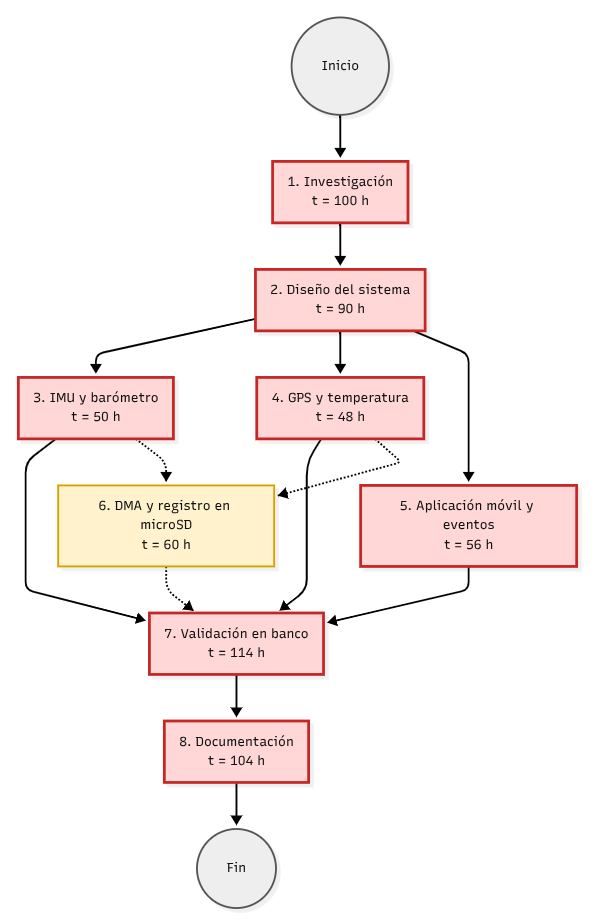
\includegraphics[width=\linewidth,height=0.75\textheight,keepaspectratio]{Figuras/AoN.png}
\caption{Diagrama \textit{Activity on Node} del proyecto.}
\label{fig:aon}
\end{figure}

El camino crítico es: \textbf{Investigación $\rightarrow$ Diseño $\rightarrow$ Aplicación móvil y eventos $\rightarrow$ Validación $\rightarrow$ Documentación}, con una duración total de \textbf{464 h} (100 h + 90 h + 56 h + 114 h + 104 h).


\clearpage
\section{11. Diagrama de Gantt}
\label{sec:gantt}

\begin{figure}[H]
\centering
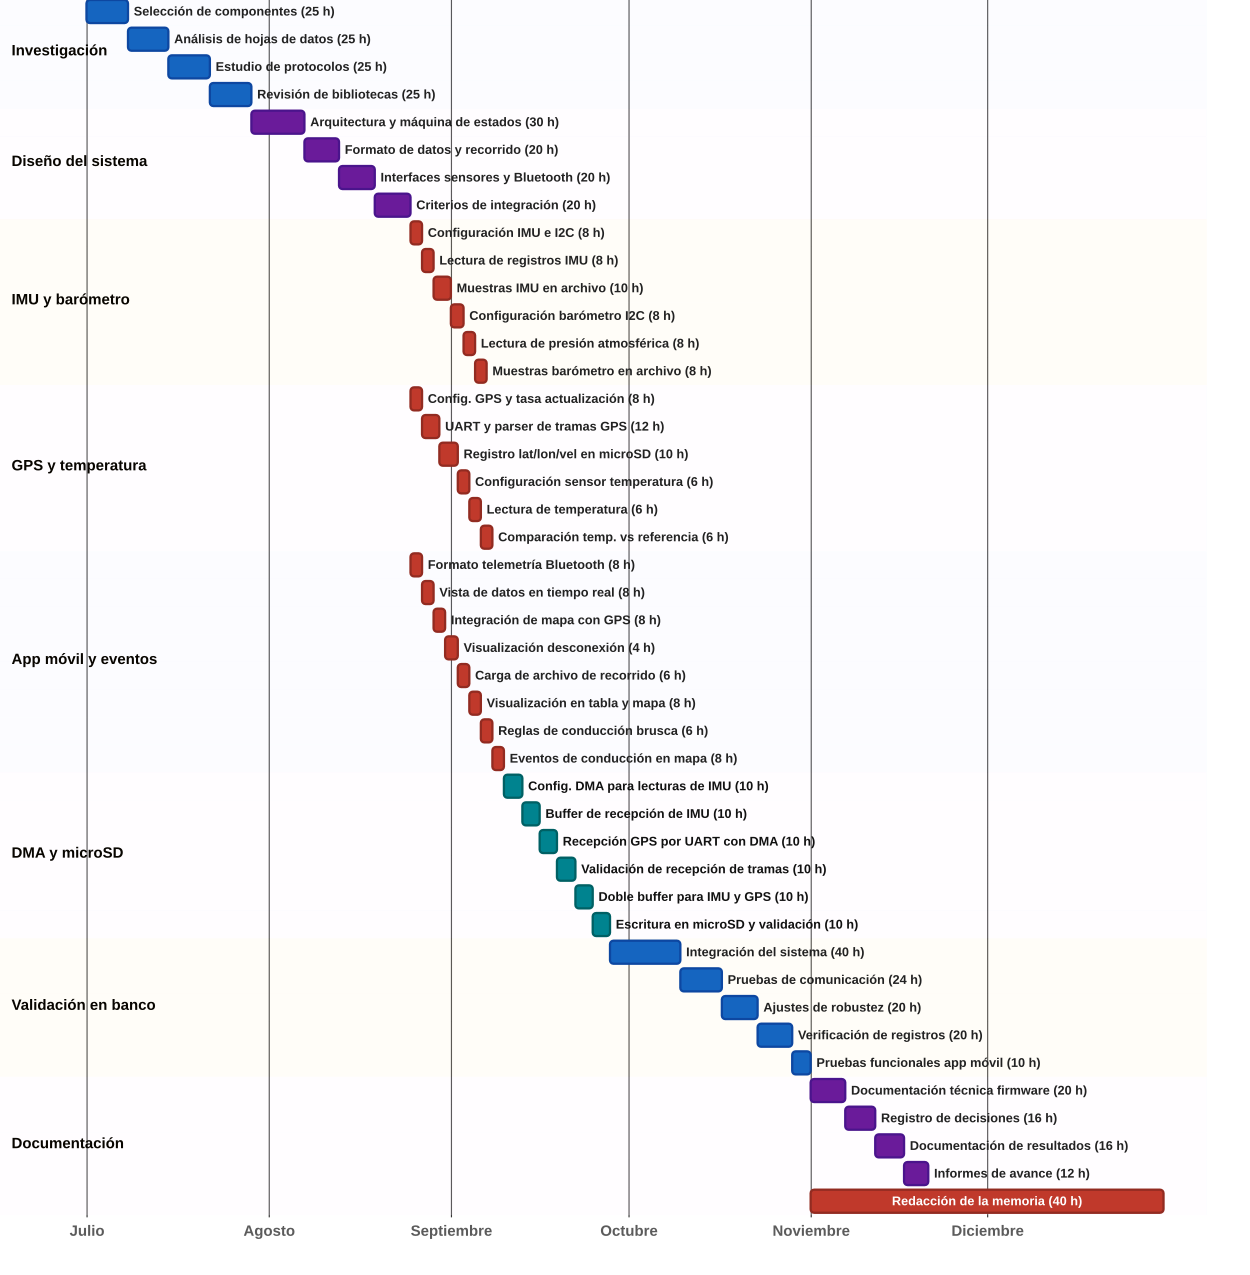
\includegraphics[width=0.85\linewidth,height=0.92\textheight,keepaspectratio]{Figuras/gantt.png}
\caption{Diagrama de Gantt del proyecto.}
\label{fig:gantt}
\end{figure}

\section{12. Presupuesto detallado del proyecto}
\label{sec:presupuesto}

En el siguiente cuadro se muestra el detalle de los costos del proyecto expresados en pesos argentinos. Los valores de componentes corresponden a precios de referencia del mercado local argentino relevados en mayo de 2026, priorizando publicaciones de Mercado Libre cuando estuvieron disponibles, y pueden variar al momento de la compra. Para los honorarios profesionales se considera una tarifa de \$ 50.000 por hora.

\begin{table}[H]
\centering
\begin{tabularx}{\linewidth}{@{}|X|c|r|r|@{}}
\hline
\rowcolor[HTML]{C0C0C0} 
\multicolumn{4}{|c|}{\cellcolor[HTML]{C0C0C0}COSTOS DIRECTOS} \\ \hline
\rowcolor[HTML]{C0C0C0} 
Descripción &
  \multicolumn{1}{c|}{\cellcolor[HTML]{C0C0C0}Cantidad} &
  \multicolumn{1}{c|}{\cellcolor[HTML]{C0C0C0}Valor unitario} &
  \multicolumn{1}{c|}{\cellcolor[HTML]{C0C0C0}Valor total} \\ \hline
Placa de desarrollo STM32 NUCLEO-F446RE &
  1 &
  \$ 40.000 &
  \$ 40.000 \\ \hline
Módulo IMU MPU6050 o equivalente &
  1 &
  \$ 10.000 &
  \$ 10.000 \\ \hline
Sensor barométrico y de temperatura BMP280 o equivalente &
  1 &
  \$ 5.000 &
  \$ 5.000 \\ \hline
Módulo GPS NEO-6M con antena &
  1 &
  \$ 15.000 &
  \$ 15.000 \\ \hline
Módulo Bluetooth BLE HM-10 o equivalente &
  1 &
  \$ 9.000 &
  \$ 9.000 \\ \hline
Módulo lector de tarjeta microSD &
  1 &
  \$ 3.000 &
  \$ 3.000 \\ \hline
Tarjeta microSD clase 10 &
  1 &
  \$ 21.000 &
  \$ 21.000 \\ \hline
Regulador DC-DC \textit{step-down} LM2596 &
  1 &
  \$ 3.000 &
  \$ 3.000 \\ \hline
Kit de prototipado, protoboard, fuente MB102 y cables &
  1 &
  \$ 19.000 &
  \$ 19.000 \\ \hline
\textit{Power bank} 10000 mAh para pruebas de campo &
  1 &
  \$ 45.000 &
  \$ 45.000 \\ \hline
Insumos menores de montaje, conectores, termocontraíble y fijaciones &
  1 &
  \$ 10.000 &
  \$ 10.000 \\ \hline
Honorarios profesionales &
  600 h &
  \$ 50.000 &
  \$ 30.000.000 \\ \hline
\multicolumn{3}{|c|}{SUBTOTAL} &
  \$ 30.180.000 \\ \hline
\rowcolor[HTML]{C0C0C0} 
\multicolumn{4}{|c|}{\cellcolor[HTML]{C0C0C0}COSTOS INDIRECTOS} \\ \hline
\rowcolor[HTML]{C0C0C0} 
Descripción &
  \multicolumn{1}{c|}{\cellcolor[HTML]{C0C0C0}Cantidad} &
  \multicolumn{1}{c|}{\cellcolor[HTML]{C0C0C0}Valor unitario} &
  \multicolumn{1}{c|}{\cellcolor[HTML]{C0C0C0}Valor total} \\ \hline
Costos indirectos estimados como 50 \% de los costos directos &
  1 &
  \$ 15.090.000 &
  \$ 15.090.000 \\ \hline
\multicolumn{3}{|c|}{SUBTOTAL} &
  \$ 15.090.000 \\ \hline
\rowcolor[HTML]{C0C0C0}
\multicolumn{3}{|c|}{TOTAL} &
  \$ 45.270.000 \\ \hline
\end{tabularx}%
\caption{Presupuesto detallado del proyecto.}
\label{tab:presupuesto}
\end{table}

El costo total del proyecto equivale a US\$ 32.336 según la cotización del Banco de la Nación Argentina al 24 de mayo de 2026.

\section{13. Gestión de riesgos}
\label{sec:riesgos}

a) Identificación de los riesgos y estimación de sus consecuencias:

A continuación se detallan los riesgos principales del proyecto. Cada riesgo se evalúa mediante severidad (S) y ocurrencia (O), con valores de 1 a 10.

Riesgo 1: demora en la adquisición de componentes o módulos comerciales.
\begin{itemize}
	\item Severidad (S): 8.\\
	Una demora en la compra o entrega de la placa de desarrollo, sensores, módulo GPS, módulo Bluetooth o microSD puede retrasar el inicio de las pruebas de integración.
	\item Ocurrencia (O): 4.\\
	Los componentes principales se consiguen en el mercado local, aunque puede existir variabilidad de stock, precios y tiempos de envío.
\end{itemize}

Riesgo 2: daño del prototipo durante pruebas en motocicleta.
\begin{itemize}
	\item Severidad (S): 8.\\
	La rotura del prototipo puede obligar a repetir tareas de integración y validación.
	\item Ocurrencia (O): 4.\\
	Las pruebas se realizarán en un entorno con vibración, movimiento y exposición a posibles desconexiones mecánicas.
\end{itemize}

Riesgo 3: integración tardía entre firmware, Bluetooth y aplicación móvil.
\begin{itemize}
	\item Severidad (S): 9.\\
	Si la integración se retrasa, puede quedar comprometida la validación funcional completa del sistema.
	\item Ocurrencia (O): 4.\\
	El proyecto combina firmware embebido, comunicación Bluetooth y una aplicación móvil, lo que incrementa la cantidad de interfaces a validar.
\end{itemize}

Riesgo 4: desempeño insuficiente del GPS o Bluetooth en condiciones reales.
\begin{itemize}
	\item Severidad (S): 7.\\
	Una mala recepción GPS o una comunicación Bluetooth inestable puede degradar la experiencia de uso y limitar las pruebas de campo.
	\item Ocurrencia (O): 4.\\
	La calidad de señal depende de la ubicación del módulo, la orientación de la antena y el entorno de prueba.
\end{itemize}

Riesgo 5: tiempo insuficiente para dominar tecnologías críticas del proyecto.
\begin{itemize}
	\item Severidad (S): 7.\\
	La falta de experiencia en DMA, manejo robusto de microSD, interpretación de GPS o desarrollo móvil puede demorar tareas técnicas clave.
	\item Ocurrencia (O): 5.\\
	El proyecto integra varias tecnologías que requieren pruebas de concepto y ajustes iterativos.
\end{itemize}

b) Tabla de gestión de riesgos: (El RPN se calcula como RPN = S x O)

\begin{table}[H]
\centering
\begin{tabularx}{\linewidth}{@{}|X|c|c|c|c|c|c|@{}}
\hline
\rowcolor[HTML]{C0C0C0} 
Riesgo & S & O & RPN & S* & O* & RPN* \\ \hline
Demora en la adquisición de componentes & 8 & 4 & 32 & 8 & 3 & 24 \\ \hline
Daño del prototipo durante pruebas en motocicleta & 8 & 4 & 32 & 8 & 2 & 16 \\ \hline
Integración tardía entre firmware, Bluetooth y aplicación móvil & 9 & 4 & 36 & 9 & 2 & 18 \\ \hline
Desempeño insuficiente del GPS o Bluetooth en condiciones reales & 7 & 4 & 28 & -- & -- & -- \\ \hline
Tiempo insuficiente para dominar tecnologías críticas & 7 & 5 & 35 & 7 & 3 & 21 \\ \hline
\end{tabularx}%
\end{table}

\FloatBarrier
\pagebreak

Criterio adoptado: se tomarán medidas de mitigación en los riesgos cuyos números de RPN sean mayores a 30.

Nota: los valores marcados con (*) en la tabla corresponden luego de haber aplicado la mitigación.

c) Plan de mitigación de los riesgos que originalmente excedían el RPN máximo establecido:

Riesgo 1: demora en la adquisición de componentes o módulos comerciales.

Plan de mitigación: realizar la compra de componentes al inicio del proyecto, identificar proveedores alternativos y priorizar módulos disponibles en el mercado local.
\begin{itemize}
	\item Severidad (S*): 8.\\
	La severidad se mantiene, ya que no contar con componentes sigue afectando el cronograma.
	\item Ocurrencia (O*): 3.\\
	La compra anticipada y la disponibilidad de alternativas reducen la probabilidad de retrasos.
\end{itemize}

Riesgo 2: daño del prototipo durante pruebas en motocicleta.

Plan de mitigación: realizar primero pruebas de banco, usar fijaciones mecánicas simples pero firmes, proteger conexiones y contar con repuestos para módulos críticos.
\begin{itemize}
	\item Severidad (S*): 8.\\
	La severidad se mantiene porque una rotura durante pruebas puede seguir requiriendo retrabajo.
	\item Ocurrencia (O*): 2.\\
	Las pruebas progresivas y la protección física reducen la probabilidad de daño.
\end{itemize}

Riesgo 3: integración tardía entre firmware, Bluetooth y aplicación móvil.

Plan de mitigación: definir un protocolo mínimo de telemetría desde el inicio, probar la aplicación con datos simulados y realizar integraciones incrementales antes de completar todos los sensores.
\begin{itemize}
	\item Severidad (S*): 9.\\
	La severidad se mantiene porque la integración completa es necesaria para validar el sistema.
	\item Ocurrencia (O*): 2.\\
	El uso de datos simulados y pruebas incrementales reduce el riesgo de descubrir problemas de integración al final del proyecto.
\end{itemize}

Riesgo 5: tiempo insuficiente para dominar tecnologías críticas del proyecto.

Plan de mitigación: realizar pruebas de concepto acotadas para DMA, microSD, GPS y Bluetooth antes de su integración final, y reutilizar bibliotecas o ejemplos probados cuando sea conveniente.
\begin{itemize}
	\item Severidad (S*): 7.\\
	La severidad se mantiene porque las tecnologías críticas siguen siendo necesarias para cumplir el alcance.
	\item Ocurrencia (O*): 3.\\
	Las pruebas de concepto tempranas reducen la incertidumbre técnica antes de comprometer el cronograma principal.
\end{itemize}

\section{14. Gestión de la calidad}
\label{sec:calidad}

Las acciones de verificación y validación se definen a partir de los requerimientos principales y de los criterios de aceptación de las historias de usuario.

\begin{itemize}
\item Requerimiento 1. Registro de datos de la IMU en microSD.
	\begin{itemize}
	\item Verificación: ejecutar una prueba de al menos 2 minutos y confirmar que el archivo generado incluye marca de tiempo, acelerómetro y giroscopio.
	\item Validación: revisar con el director que los datos registrados sean consistentes con el movimiento aplicado al sensor.
	\end{itemize}
\item Requerimiento 2. Registro de datos del barómetro.
	\begin{itemize}
	\item Verificación: generar un archivo de prueba en microSD y confirmar que cada registro incluya marca de tiempo y presión atmosférica.
	\item Validación: comparar las lecturas con condiciones ambientales esperadas durante la prueba.
	\end{itemize}
\item Requerimiento 3. Registro de posición y velocidad GPS.
	\begin{itemize}
	\item Verificación: recibir tramas GPS válidas durante una prueba de al menos 2 minutos y registrar latitud, longitud y velocidad.
	\item Validación: comprobar que la posición registrada sea coherente con la ubicación de prueba.
	\end{itemize}
\item Requerimiento 4. Registro de temperatura.
	\begin{itemize}
	\item Verificación: registrar temperatura en microSD con marca de tiempo y unidades en grados Celsius.
	\item Validación: comparar la lectura contra una referencia de banco.
	\end{itemize}
\item Requerimiento 5. Uso de DMA para lecturas de IMU.
	\begin{itemize}
	\item Verificación: confirmar que la IMU se lea usando DMA hacia un buffer en RAM sin copia manual de cada muestra por CPU.
	\item Validación: verificar que durante una prueba no se detecten errores de transferencia y que la cantidad de muestras coincida con la frecuencia configurada.
	\end{itemize}
\item Requerimiento 6. Recepción GPS con DMA.
	\begin{itemize}
	\item Verificación: confirmar que las tramas GPS se reciban por UART con DMA hacia memoria.
	\item Validación: evaluar recepción de tramas completas y manejo de tramas inválidas sin bloqueo del sistema.
	\end{itemize}
\item Requerimiento 7. Escritura en microSD con doble buffer.
	\begin{itemize}
	\item Verificación: comprobar que mientras un buffer se escribe en microSD el otro continúe recibiendo datos nuevos.
	\item Validación: ejecutar una prueba de al menos 2 minutos sin pérdida de muestras y confirmar persistencia del archivo.
	\end{itemize}
\item Requerimiento 8. Visualización móvil de telemetría en tiempo real.
	\begin{itemize}
	\item Verificación: confirmar que la aplicación muestre altitud, latitud, longitud, velocidad, temperatura y ángulo de inclinación.
	\item Validación: verificar que ante una interrupción de comunicación se informe la pérdida de conexión al usuario.
	\end{itemize}
\item Requerimiento 9. Visualización de posición actual en mapa.
	\begin{itemize}
	\item Verificación: confirmar que la posición se actualice con cada dato GPS válido.
	\item Validación: comprobar que ante errores de lectura se informe que la posición no está disponible.
	\end{itemize}
\item Requerimiento 10. Carga de recorridos almacenados.
	\begin{itemize}
	\item Verificación: cargar un archivo exportado y mostrar sus datos sin conexión con la motocicleta.
	\item Validación: comprobar que ante un archivo con formato inválido la aplicación muestre un mensaje de error.
	\end{itemize}
\end{itemize}

\section{15. Procesos de cierre}    
\label{sec:cierre}

Al finalizar el proyecto se realizará una reunión de cierre entre el responsable del proyecto y el director del Trabajo Final. El objetivo será revisar los resultados obtenidos, contrastarlos con la planificación inicial y registrar las lecciones aprendidas.

\begin{enumerate}
	\item Análisis del cumplimiento del plan de proyecto.

	El responsable será el \authorname. Se comparará la planificación original contra la ejecución real del proyecto, considerando alcance, cronograma, presupuesto, riesgos y entregables. Para ello se revisarán el diagrama de Gantt, el registro de tareas realizadas, los costos finales y los resultados de las pruebas de validación.

	Como resultado de esta actividad se documentarán los desvíos principales, sus causas y las acciones tomadas durante el desarrollo.

	\item Identificación de técnicas y procedimientos útiles e inútiles.

	Se revisarán las decisiones técnicas aplicadas durante el proyecto, incluyendo el uso de la máquina de estados, el manejo de sensores, la escritura en microSD, la comunicación Bluetooth, el uso de DMA y la estrategia de pruebas.

	Se identificarán las prácticas que resultaron útiles para el avance del proyecto y aquellas que no aportaron el resultado esperado. También se registrarán los problemas encontrados, las soluciones aplicadas y las recomendaciones para futuros desarrollos similares.

	\item Archivado de la documentación del proyecto.

	El responsable organizará y respaldará toda la documentación generada durante el proyecto. Se incluirán el código fuente, diagramas, registros de pruebas, informes de avance, memoria final, presupuesto actualizado y material utilizado para la presentación.

	La documentación quedará almacenada en el repositorio del proyecto y en una copia local de respaldo.

	\item Presentación pública y agradecimiento a los interesados.

	El responsable redactará la memoria final del Trabajo Final, incorporando la descripción del sistema, las decisiones de diseño, los resultados de validación y las conclusiones. Luego se realizará la presentación pública en el marco de la Carrera de Especialización en Sistemas Embebidos.

	En el marco de dicha presentación, el responsable del proyecto organizará un agradecimiento formal al director, al jurado y a las personas que hayan colaborado durante el desarrollo.

	El financiamiento de cualquier gasto asociado será asumido por el responsable del proyecto.
\end{enumerate}


\end{document}